\chapter{Problem Formulation} \label{Chapter3}

As discussed at length in \textit{Chapter 2}, the rapid advancement of security threats in response to technological developments and innovations makes it crucially important for mitigation techniques and tools to keep pace. One thing is abundantly clear: That there is an urgent need for re-evaluation of current best-practice in cybersecurity defences, particularly for critical service infrastructures whose general lack of implemented security mechanisms is positively dangerous. It is this consideration that is at the heart of formulating objectives for this research.

\textit{Section \ref{IdentifiedChallenges}} explores a number of the major challenges identified in \textit{Chapter 2}, seeking out the heart of the issues and hypothesising about how these can be resolved in tandem.

\textit{Section \ref{ProposedWork}} addresses the identified challenges in the formulation of proposed work for this research, and outlines the basis of the research objectives. How these research objectives will be addressed in practise is the subject of \textit{Chapter 4}.


%
%
% 	SECTION 1: CHALLENGES IDENTIFIED
%
%

\section{Identified Challenges \label{IdentifiedChallenges}}

A number of challenges currently facing the security of modern infrastructures and systems were explored in \textit{Chapter 2}. The challenges found to be of most interest to this research are outlined in the following subsections.


\subsection{Incident Monitoring in Critical Service Infrastructures}
As explained in the context of the WannaCry ransomware attacks on the NHS in \textit{Section \ref{WannaCryNHSCase}}, IT systems in many organisations are comparable to a \textit{black-box system}\footnote{This is a term commonly used in control systems theory meaning that the inputs and outputs of a system are known whilst the internal workings are not.}, an illustration of which can be seen in figure \ref{fig:Images/black_box.png}. Such a system gives no indication of what is happening internally until it begins to behave unexpectedly, meaning that when issues arise they are difficult to diagnose and almost impossible to resolve. However, ineffective feedback mechanisms are often as bad as having no mechanism in place: Passive mechanisms like firewalls are imprecise in their suspection of malicious activity, meaning that when a significant event does occur it can easily go unnoticed. \cite{Voronkov:2017:SLR:3161158.3130876} It is crucially important that \textit{effective} feedback mechanisms are employed which are simple to use and capable of communicating key information to those who can act upon it.


%\includewidefigure{Images/black_box.png}{Illustration of a Black-Box System}{An illustration of a black-box system, where a known input \textit{f(x)} is provided to the system, unknown operations are performed on it, and a known output \textit{g(x)} is generated as a result.}{Images/black_box.png}

\begin{figure}[ht]
      \centering
      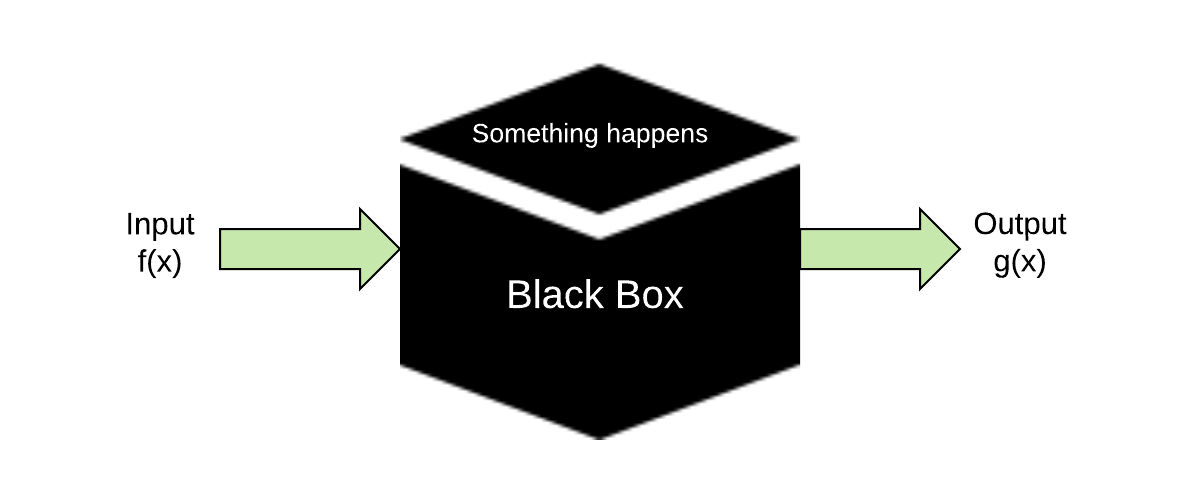
\includegraphics[width=175mm, scale=1]{Images/black_box.png}
      \caption{Illustration of a Black-Box System} 
      \medskip
	  \small
		An illustration of a black-box system, where a known input \textit{f(x)} is provided to the system, unknown operations are performed on it, and a known output \textit{g(x)} is generated as a result.
\label{fig:Images/black_box.png}
\end{figure}

It is obvious that in order to implement effective threat mitigation mechanisms, the most relevant risks to that system must first be understood: Something that was highlighted in an interview with Stuart Reed, senior director at NTT security, who argues that ''the best starting place is to understand where... risks come from''. \cite{MANSFIELDDEVINE201716} To illustrate this, consider critical service infrastructures such as the NHS: These are most at risk from those with a political motivation to do damage to a nation-critical infrastructure, such as nation-state attackers. While such infrastructures generally rely on firewalls which may protect against script-kiddies and other unsophisticated attackers, nation-states generally employ sophisticated technical attackers who are capable of discovering entirely new flaws and exploits in systems. This motivates and highlights the need for a technology that is able to provide intelligence on these active, dynamic threats for critical service infrastructures.


\subsection{The Need for Active Defence Mechanisms}
%As has been highlighted by their success in a number of the \textit{closely related projects} in \textit{Section \ref{CloselyRelatedWork}}, 
As discussed in \textit{Section \ref{ChallengesForFirewalls}}, although the use of passive intrusion detection technologies such as firewalls hold an important place in securing IT systems, they have limited diagnostic capabilities since they can only mitigate against \textit{known threats}. In an analogy comparing cybersecurity to health, Fred Schneider explains that ''as with medical problems, some attacks are best addressed in a reactive way''. \cite{Schneider11_BlueprintForScienceOfCybersecurity} 

Honeypot-driven solutions are promising in what they can offer with regards to active network defence and rapid incident response. Modern IT infrastructures are sorely in need of such \textit{adaptive} approaches to defence: Defence mechanisms that, in the face of uncertainty about the nature of attacks, can continue to provide threat mitigation. It is clear from the discussion provided in \textit{Section \ref{HoneypotsSection}} that honeypot solutions have the ability to address this requirement.

\begin{itemize}
\item The information that honeypots can capture enables continuous improvement of infrastructure design and defences;
\item The low number of false positives that result from honeypots make identifying threats straight-forward: All logged events can generally be assumed to be threats;
\item Honeypots are capable of alerting first-responders to highly-probable threats as soon as they occur, enabling rapid response before an attack has the opportunity to spread.
\end{itemize}

However, these benefits are identified in recognition of the fact that the widespread deployment of honeypot-based systems to-date has been impeded by the maintenance overhead that they incur for system administrators, as was identified by the developers of Deutsche Telekom's TPot as outlined in \textit{Section \ref{AboutTPot}}. In order for such a system to be practical and feasible to deploy in a production system, it must be:

\begin{enumerate}
    \item Inexpensive to deploy, operate and maintain;
    \item Effective and reliable in securing a network;
    \item Simple to use.
\end{enumerate}
    
In order to be viable for widespread adoption as a security service, a honeypot-based deployment solution must address all of these requirements.
	
\subsection{The Effectiveness of Honeypots in Enticing Attacks}
%This is in relation to how effectively honeypots are designed in order to entice attacks, which is a crucial element to their success.
As identified from the closely related work explored in \textit{Section \ref{CloselyRelatedWork}}, although there has been excellent progress made in the enhancement of honeypot design so that attack sessions are prolonged and more attack data is captured for analysis, there is little conclusive research found regarding how to enhance the design of honeypots in order to initiate the interest of attackers. 

In almost all research found, there was a heavy focus on encouraging the prolonged interaction of attackers with honeypots rather than on attracting that interaction in the first place. \cite{CowrieWebsite} \cite{IoTPot2016} \cite{IoTCandyJar} \cite{Dowling2017} Dowling \textit{et al.} explored some interesting measures to entice attackers seeking to compromise Zigbee devices, but the impact that these measures had on the number of attacks attracted was not a metric of interest in their research. \cite{Dowling2017}

The effectiveness of honeypot-based technologies in defending systems is influenced greatly by their ability to attract attacks away from valuable systems in the environment they serve to protect. Understanding how honeypots can be designed to be as irresistible as possible to attackers would further their adaptivity in rapidly alerting first responders to the fact that they have been attacked, allowing action to be taken before a subsequent attack is targeted at valuable systems.


%
%
% 		SECTION 2: PROPOSED WORK
%
%

\section{Proposed Work} \label{ProposedWork}

It is clear that taking an active approach to mitigating risks to critical service infrastructures is the way forward, and that the capabilities of honeypots can aid greatly in achieving this. Though there are a number of existing approaches both in research and production outlined in \textit{Section \ref{CloselyRelatedWork}} that have contributed excellent work towards such a solution, there exists no one solution which can provide a practical, feasible means of employing active network defence as a single networked deployable unit.

Given the challenges identified in \textit{Section \ref{IdentifiedChallenges}}, two research objectives were formulated as a proposal to tackle them.

\subsection{Objective 1: A Honeypot-Driven Cyber Incident Monitor for Critical Service Infrastructures} \label{Objective1}

This objective addresses the need for a feasible active intrusion detection solution to enable rapid response in critical service infrastructures by enabling action to be taken on threats with minimal operational overhead. 

The requirements of such a solution include:

\begin{enumerate}
\item A deployment solution that is cost-effective, quick to deploy and quick to scale, whilst compatible with existing IT infrastructure. 
\item A number of highly-attractive honeypots, which can effectively lure attackers away from valuable machines in the network in which they are deployed. 
\item A centralisation point for data collected from any deployed honeypots, such that administrators may be given a holistic view of their system in order to facilitate them in making quick, well-informed decisions.
\item An effective and reliable alert system, such that the key parties can be alerted as soon as possible after a threat event is detected by the system.
\end{enumerate}

The constituent components of such a system are addressed in the following sections.

\subsubsection{Honeypots for Active Network Defence}
As outlined at length in \textit{Section \ref{HoneypotsSection}}, honeypots enable the identification of vulnerabilities and flaws in the system in which they are deployed and are capable of mitigating against risks that were previously unknown to those administering the system, unlike passive defence mechanisms like firewalls. This makes them an obvious choice for the implementation of active network defence in critical service infrastructures.

In the proposed incident monitoring system, the use of a number of honeypots in a honeynet configuration has been identified as a ideal approach to providing effective incident monitoring. There are multiple benefits of a honeynet-based approach here, including the potential to study attack propagation through a network and the fact that there is an increased honeypot attack surface to distract an attacker away from valuable systems in the same environment. The honeypots in the proposed system would act as sensors, providing a feedback mechanism regarding threat events in the network by logging attack activities for analysis.



\subsubsection{Containerised Honeypots}
Containers have been identified as an effective deployment option for the proposed system, given the properties that were outlined in \textit{Section \ref{SecurityThroughContainerisation}}, since they cater for many of the requirements of a scalable honeypot-based incident monitoring system as outlined in the previous section.

By deploying honeypots in inter-networked containers it becomes possible to provide a flexible, low-cost, low-maintenance deployment solution for organisations. A single container will only use a relatively small proportion of a machine's CPU power and storage, and a number of containers on a single host can use the same physical network interface whilst implementing their own independent network stack. \cite{LXCsForDeceptiveHoneypots2017} Importantly, any container can be deployed and removed with minimal operational overhead because of their portable configuration. In the case of critical service infrastructures, using such an architecture would enable recovery of any containerised component of the system after compromise with minimal downtime. 

From the perspective of overhead and maintenance, containers are an excellent choice as a hosting platform for applications in today's IT infrastructures. The migration of security applications to container-based architectures is both beneficial and essential for organisations hosting their infrastructure in containers: The success of containerised honeypots in the TPot platform illustrates this. \cite{TPotWebpagev17} As well as this, containers enable a degree of reproducibility not usually achievable in computer science research, as pointed out by Cito \textit{et al.}. \cite{ReproducableResearchEnvironmentsContainers} All of these benefits give a strong basis for the use of containers in hosting a honeypot-driven solution. 



\subsubsection{Visualisation of Honeypot-Generated Data}
Analysis of honeypot data is simplified greatly through use of visualisation tools, which enable classification and visualisation of complex attack data in order to make meaningful deductions. 

As part of a honeypot-driven incident monitoring solution, it is clear that information gathered from honeypots would benefit from being aggregated, analysed and visualised in a central management system that consolidates the data and perform processing operations on it before making it available to a user: Both the MHN and TPot projects exemplify this approach. \cite{TPotWebpagev17} \cite{ModernHoneyNetworkLaunchAnnouncement}

Such a management system is a crucial component of the cyber incident monitoring system, where attack data is gathered centrally and made accessible to system administrators who require a holistic view of the state of the system. A management system performing this function should be directly reachable by the honeypots, but obscured from attackers within them.  


\subsubsection{Notification System for Threat Events}
The challenges faced in the aftermath of the WannaCry ransomware infection of NHS systems have illustrated the importance of having a feedback mechanism in place, which is capable of notifying first-responders in the event of undesirable behaviour being detected. An effective cyber incident monitor should provide this feedback mechanism, allowing threat data to be presented to those who can act on it as soon as it is detected.


\subsection{Objective 2: A Proposal for Adaptive Honeypots} \label{Objective2}

It is clear that the effectiveness of honeypots in intrusion detection depends heavily on their design, which in turn depends on the context of their deployment and the value that they are required to deliver. The single point of commonality between all honeypot deployments is that they must be \textit{adaptive} in order to deceive attackers effectively, assisting them in what they believe to be the successful progression of their attack whilst quietly monitoring their actions. 

This need for adaptivity is beginning to be addressed in research more commonly, but there are gaps in current research that have provide an opportunity for improvement. In particular, all of the closely related honeypot projects identified in \textit{Section \ref{RelatedHoneypotProjects}} which address the adaptivity of honeypots focus on approaches to \textit{maintaining} the interest of an attacker, rather than on initiating the interest in the first place. \cite{CowrieWebsite} \cite{IoTPot2016} \cite{IoTCandyJar} Designing adaptive honeypots such that they advertise the most commonly sought-after characteristics of victim systems is a problem of major interest.
% However, IoTCandyJar does not address what characteristics of their honeypots attracted the attackers in the first place: Their implementation is more focused on maintaining interest than initiating it.

%\begin{figure}[ht]
%     \centering
%      \includegraphics[width=100mm, scale=0.6]{Images/Baseline__SoA__proposed_and_optimal_solutions.png}
%      \caption{add caption}
%      \medskip
%	  \small
%		An illustration of the relative improvement that is possible in the design of a solution. In recognition of the fact that the theoretical optimal solution is not attainable, one would strive to improve upon the current state-of-the-art and devise a solution that is as close as possible to the theoretical optimum.
%      \label{TheoreticalOptimalSolution}
%\end{figure}

%\includefigure{TheoreticalOptimalSolution}{Improving upon a baseline implementation}{An illustration of the relative improvement that is possible in the design of a solution. In recognition of the fact that the theoretical optimal solution is not attainable, one would strive to improve upon the current state-of-the-art and devise a solution that is as close as possible to the theoretical optimum.}{Images/Baseline__SoA__proposed_and_optimal_solutions.png}


\subsubsection{Measuring the Effectiveness of Honeypot Characteristics} \label{BenefitsForUsingHoneynetForExperiments}
Conducting a robust evaluation of the effectiveness of particular honeypot characteristics in attracting the interest of attackers is an interesting but difficult problem. The effectiveness of a honeypot is difficult to quantify, but it is clear than an effective honeypot will provide effective intrusion detection and, depending on the context of its deployment, capture relevant attack data in a certain level of detail.

Honeypot effectiveness can potentially be measured through such properties as the number of attacks that are attracted, the number of true positives detected, the ability to deduce attacker motivation based on data captured, etc. \cite{Nawrocki2016} Credible measurement of any of these properties is largely dependent on maintaining a consistent research environment within which relative performance can be evaluated accurately.

A honeynet is an effective way of accurately and simultaneously measuring the appeal of certain characteristics of honeypots in experiments, since multiple characteristics can be trialled in the same environment over the same period of time. By using a honeynet configuration in the research environment, data can be captured from multiple honeypots under the same environmental conditions, and the relative performance based on slightly different configurations can be measured. 


\subsubsection{Targeted Honeypots for the Internet of Things}
From the outset of this research, one of the most interesting and active categories of botnet identified was that of IoT botnets, a revolutionary and recent phenomenon which is cause for serious concern. 

Proposing an approach to designing adaptive honeypots with a focus on making them maximally attractive to IoT botnets would contribute to current knowledge of these attackers by understanding more about their preferred vulnerabilities and target systems. The configurability and informative capabilities of honeypots makes them an attractive option in this regard. Targeting these attackers in the design and implementation of the proposed system would be a valuable additional contribution to the field of security as an application of the cyber incident monitor.





